%%%%%%%%%%%%%%%%%%%%%%%%%%%%%%%%
% Chap 3.     CoNAC for Uncertain Euler-Lagrange Systems Under Weight Constraints
%%%%%%%%%%%%%%%%%%%%%%%%%%%%%%%%

\chapter{
    CoNAC for Uncertain Euler-Lagrange Systems Under Weight Constraints
} \label{chapter3}

%%%%%%%%%%%%%%%%%%%%%%%%%%%%%%%%
\section{Introduction} 
%%%%%%%%%%%%%%%%%%%%%%%%%%%%%%%%

In this chapter, a novel constrained optimization based neuro-adaptive control (CoNAC) is presented for uncertain Euler-Lagrange systems with a weight norm constraint. 
As presented in Chapter \ref{chap1:sec:example}, one of the common issues in neuro-adaptive control (NAC) is that the boundedness of neural network’s (NN) weights is not guaranteed.
Since the amplitude of control input of NAC is dependent on the weights, the unbounded weights may lead to instability and severe safety issues. 
The satisfaction of the boundedness of the weights are reformulated into weight norm constraints, which are then incorporated into the CoNAC.

%%%%%%%%%%%%%%%%%%%%%%%%%%%%%%%%
\section{Problem Formulation}
%%%%%%%%%%%%%%%%%%%%%%%%%%%%%%%%

Consider an uncertain Euler-Lagrange system modeled as
\begin{equation}
    M(q)\ddot q + C(q,\dot q)\dot q + G(q) + F(q) = \tau
    \label{chap3:eq:sys1}
\end{equation}
where $q\in \R^n$ and $\tau\in\R^n$ denotes the generalized coordinate and the control input, respectively; $M(q)\in\R^{n\times n}$, $C(q,\dot q)\in\R^{n\times n}$, and $G(q)\in\R^{n}$ denote the unknown system function matrices; and $F(q)\in\R^{n}$ denotes the external force.

Using the user-designed matrices $M_0>0,C_0$ and $G_0$, \eqref{chap3:eq:sys1} can be represented as 
\begin{equation}
    M_0\ddot q+C_0\dot q+G_0 = \tau + f(q,\dot q,\ddot q)
    \label{chap3:eq:sys2}
\end{equation}
where $f(q,\dot q,\ddot q) \triangleq -(M-M_0)\ddot q-(C-C_0)(q,\dot q)\dot q -(G-G_0) -F(q)$ denotes the residual unknown term.

As presented in Section \ref{chap1:sec:example}, the parameter drift (\ie the weights of NNs can diverse) may occur due to the lumped disturbance term.
Hence, the objective of the control design is to make $q$ track the continuously differentiable desired trajectory $q_d(t):\R\to \R^n$ under the unknown terms $f$ while ensuring boundedness of weights of NN in the controller.

%%%%%%%%%%%%%%%%%%%%%%%%%%%%%%%%
\section{Exiting Works for Boundedness of Weights} 
%%%%%%%%%%%%%%%%%%%%%%%%%%%%%%%%

Most studies modify their adaptation laws to ensure the boundedness of the weights.

\subsection{Projection Operator} \label{chap3:sec:proj}

In \cite{RN13, RN11, RN21}, the projection operator is utilized to prevent the weight divergence, by projecting the adaptation direction on some convex set of the weights.
The projection operator is defined in \cite[Appendix E, eq.~(E.4)]{RN7} and represented as
\begin{equation}
    \text{Proj}_\Omega(y)
    =
    \begin{cases}
        \Gamma y
        &
        \begin{aligned}
            &\text{if }x\in\Omega
            \text{ or if }\\
            &x\in\delta\Omega
            \text{ and }
            \nabla c^T\Gamma y\ge0
        \end{aligned}
        \\
        \Gamma y
        -
        \Gamma
        {\nabla c\nabla c^T\over \nabla c^T \Gamma \nabla c}
        \Gamma y
        &
        \text{otherwise}
    \end{cases}
    \label{chap3:eq:proj}
\end{equation}
where $\Gamma=\Gamma^T>0$ is adaptation gain matrix and $y\in\R^n$ denotes the update direction of optimization variable $x\in\R^n$.
Moreover, $\Omega\triangleq \{x\ \vert\ c(x)\le 0\}$ denotes a convex set defined by $c(\cdot)$ is a convex function and $\delta\Omega$ denotes a boundary of $\Omega$.
The convex function $c(\cdot)$ is typically selected as $x^Tx\le \bar x^2$ where $\bar x\in\R_{>0}$ is a maximum norm of $x$.
However, in the literature, the projection operator is only applied to theoretically guarantee the boundedness of the weights, by selecting the convex set as large as possible.
This is because, the authors attempts to estimate the globally ideal weights whose magnitude is unknown.

\subsection{
    \texorpdfstring{$\sigma$}{σ} and \texorpdfstring{$\epsilon$}{ε}-modifications
} 
%  \texorpdfstring{$\mu=0$}{μ=0}

In adaptive control theory, the $\sigma$-modification \cite{RN19} and the $\epsilon$-modification \cite{RN18, RN46} are widely used to regulate the magnitude of the weights by adding a stabilizing function in the adaptation law as follows:
\begin{equation}
    y_\sigma = \Gamma (y+\lambda x)
    ,
    \quad
    y_\epsilon = \Gamma (y+\rho\Vert e\Vert x)
\end{equation}
where $y_i,\ i\in[\sigma,\epsilon]$ denote adaptation laws of $\sigma$-modification and $\epsilon$-modification, respectively, $e$ denotes tracking error, and $\lambda$ and $\rho$ denote parameters of $\sigma$-modification and $\epsilon$-modification, respectively.
These methods make the invariance set of the estimation error of the weights over time.
The existing methods have shown their effectiveness in ensuring the boundedness of the weights via numerical simulations.
However, the weights are biased to the origin by the stabilizing function, which may degrade the performance of the controller.
This means that there is a trade-off between the boundedness of the weights and the optimality of the weights.
Moreover, they lack theoretical analysis regarding the optimality of the adapted weights.

Interestingly, similar approaches that regulate the magnitude of the weights have also been introduced in the deep learning literature.
One of the approaches is $L_2$-regularization, which adds the squared magnitudes of the weights to the objective function \cite{RN34, RN36}.
Then, the adaptation process attempts to reduce not only the original objective function, but also the magnitude of the weights.
By regulating the magnitude of the weights, the stability of the adaptation process can be enhanced, and overfitting can be prevented.
However, $L_2$-regularization also involves same limitations as $\sigma$ and $\epsilon$-modifications.

%%%%%%%%%%%%%%%%%%%%%%%%%%%%%%%%
\section{CoNAC with Weight Norm Constraint} \label{chap3:problem} 
%%%%%%%%%%%%%%%%%%%%%%%%%%%%%%%%

Without loss of generality a single hidden layer neural network (SHLNN) is utilized in this chapter for better intuition and simplicity. 
Note that SHLNN is the simplest case of DNN presented in Section \ref{chap2:sec:DNN}.
The architecture of the CoNAC is illustrated in Fig.~\ref{chap3:fig:ctrl}, consisting of: a reference generator, the SHLNN that functions as NAC, and a weight optimizer for the SHLNN. 
The reference generator is designed based on backstepping control (BSC), presented in previous Section \ref{chap2:sec:ctrl} , to generate a tracking reference for both $q$ and $\dot q$.

\begin{figure*}[t]
    \centering
    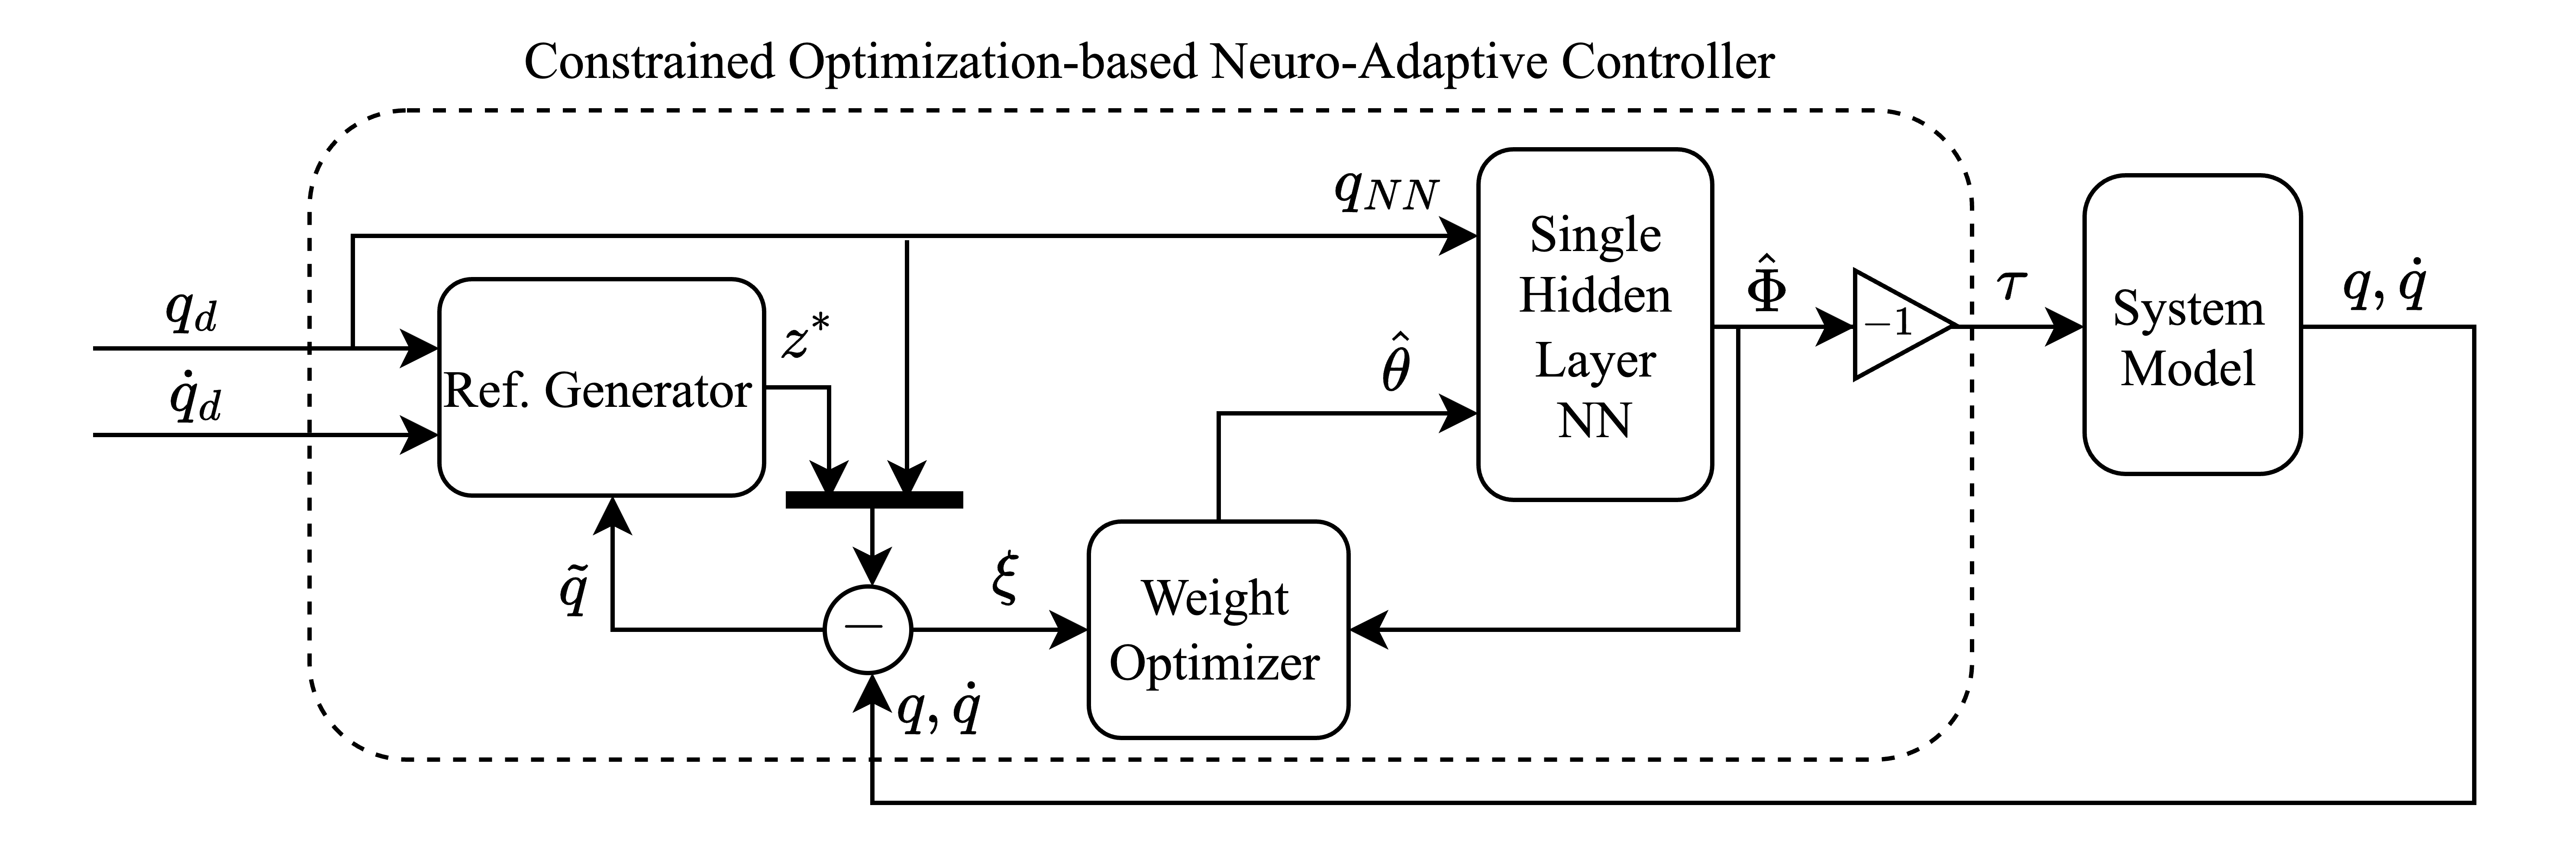
\includegraphics[width=0.9\linewidth]{imgs/ControllerChap3.drawio.png}
    \caption{Architecture of the constrained optimization-based neuro-adaptive controller (CoNAC).}
    \label{chap3:fig:ctrl}
\end{figure*}

\subsection{Control Law Development} \label{chap3:sec:ctrl_dev}

The system dynamics \eqref{chap3:eq:sys2} can be represented as
\begin{equation}
    \begin{aligned}
        \dot {q} &= {z},\\
        \dot {z} &= -M_0^{-1} C_0 {z}-M_0^{-1} G_0+M_0^{-1} h(\tau) + M_0^{-1} f,
    \end{aligned}
    \label{chap3:eq:x_dyna}
\end{equation}
where ${z}\triangleq \dot q$.

Consider the Lyapunov function ${\mathcal V}_{c1}\triangleq(1/2){\tilde q}^T  {\tilde q}$, where ${\tilde q}\triangleq {q}-{q_d}$ represents the tracking error between the actual trajectory ${q}$ and the desired trajectory $q_d$. 
The desired trajectory of ${z}$, ensuring $\dot {\mathcal V}_{c1}={\tilde q}^T  ({z}-\dot {q_d})<0$ is 
\begin{equation}
    {z^*} \triangleq -{k_q}{\tilde q} + \dot q_d,
\end{equation}
which functions as the reference generator with control gain ${k_q} \in\R_{>0}$. The tracking error of ${z}$ relative to the desired trajectory ${z^*}$ is defined as
\begin{equation}
    {\tilde z} \triangleq {z} - {z^*} = {z} - (-{k_q}{\tilde q} + \dot q_d).
    \label{chap3:eq:e2}
\end{equation}

Next, consider the Lyapunov function ${\mathcal V}_{c2}\triangleq {\mathcal V}_{c1} + (1/2) {\tilde z}^T  {\tilde z}$.
Its time derivative is
\begin{equation}
    \begin{aligned}
    \dot {\mathcal V}_{c2} &=
    {\tilde q}^T  (-{k_q}{\tilde q}+{\tilde z}) +{\tilde z}^T  (-M_0^{-1} C _0{z} -M_0^{-1} G_0\\
    &\quad
    +M_0^{-1}h(\tau)+M_0^{-1} f- \dot z^*)\\
    &= -{k_q}{\tilde q}^T  {\tilde q} -{k_z}{\tilde z}^T  {\tilde z} +{\tilde z}^T  ({k_z}{\tilde z}+{\tilde q}\\
    &\quad-M_0^{-1} C_0{z} -M_0^{-1} G_0+M_0^{-1} h(\tau)+M_0^{-1} f- \dot z^* )
    \end{aligned}
\end{equation}
with control gain ${k_z}\in\R_{>0}$. 
The stabilizing control law, which does not account for weight norm and input constraints, is defined as follows:
\begin{equation}
    \tau^* \triangleq-M_0\cdot ({k_z}{\tilde z})+ 
    ( 
        -M_0{\tilde q}+C_0{z}+G_0-f+M_0 \dot z^*
    )
    .
    \label{chap3:eq:desired_control}
\end{equation}
This control law ensures that the time derivative of the Lyapunov function is negative definite, as $\dot {\mathcal V}_{c2} = -{k_q}{\tilde q}^T  {\tilde q}-{k_z}{\tilde z}^T  {\tilde z}<0$, in the absence of any constraints. 
However, the control law $\tau^*$ cannot be realized in practice because the lumped system uncertainty function $f$, which accounts for unmodeled dynamics and disturbances, is not available.

As introduced in Section \ref{chap2:sec:DNN}, the SHLNN which is simple version of DNN is represented as 
\begin{equation}
    \Phi({q_{NN}};\theta)\triangleq V_1^T\phi(V_0^T{q_{NN}})
\end{equation}
where ${q_{NN}}\in\R^{l_0+1}$ denotes the NN input vector, $V_i\in\R^{(l_i+1)\times l_{i+1}},\ i\in[0,1]$ denotes the weight matrix of $i\textsuperscript{th}$ layer and $\phi:\R^{l_1}\to\R^{l_1+1}$ denotes the activation function layer.
The element-wise activation function layer consists of nonlinear function $\sigma(\cdot)$ and augmented $1$ to combine the bias term in weight matrix (\ie $\phi(x) = [\sigma(x_{(1)}),\cdots, \sigma(x_{(l_1)}), 1]^T$).
For further simplicity, let $\theta\triangleq[\theta_1^T,\theta_0^T]^T\in\R^{\Xi}$ denote the total weight vector, where $\theta_i\triangleq \text{vec}(V_i)\in\R^{\Xi_i}$ denote the vectorized weights.
$\Xi_i=(l_i+1)\cdot l_{i+1}$ and $\Xi=\Xi_0+\Xi_1$ denote the number of each layer and total weights, respectively.

Using this SHLNN, the desired controller $\tau^*$ can be approximated through ideal weight vector $\theta^*$ for a compact subset $\Omega_{NN}\in\R^{l_0+1}$ to $\epsilon$-accuracy according to Theorem \ref{chap2:thm:uni_approx} such that $\sup_{{q_{NN}}\in\Omega_{NN}} \Vert\Phi({q_{NN}};\theta^*) - \tau^*\Vert=\epsilon<\infty$.
The ideal weight vector $\theta^*$ is typically assumed to be bounded.
In this thesis, $\theta^*$ is defined as a local optimal point, rather than a global optimal point.
Then using the estimated weight vector $\hat\theta=[\hat\theta_1^T,\hat\theta_0^T]^T$ of $\theta^*=[\theta_1^{*T},\theta_0^{*T}]^T$, the desired controller $\tau^*\approx -\Phi(q_{NN};\theta^*)-\epsilon$ can be approximated as follows:
\begin{equation}
    \tau \triangleq -\Phi({q_{NN}};\hat\theta)
    .
    \label{chap3:eq:approx_control}
\end{equation}
For further sections, let $\Phi^*\triangleq\Phi({q_{NN}};\theta^*)$ and $\phi^* \triangleq\phi(V_0^{*T}{q_{NN}})$, and $\hat\Phi\triangleq\Phi({q_{NN}};\hat\theta)$, $\hat\phi \triangleq\phi(\hat V_0^{T}{q_{NN}})$ and $\hat\phi' = \partial \hat\phi/\partial (\hat V_0^Tq_{NN})$.

Using \eqref{chap3:eq:x_dyna}, \eqref{chap3:eq:e2}, \eqref{chap3:eq:desired_control}, and \eqref{chap3:eq:approx_control}, the error dynamics can be derived as
\begin{equation}
    \begin{aligned}
        \dot {\tilde q} = & -{k_q} {\tilde q} + {\tilde z} \\
        \dot {\tilde z} = & -{\tilde q} -{k_z} {\tilde z} + M_0^{-1} (\Phi^*-\hat\Phi+\epsilon).
    \end{aligned}
    \label{chap3:eq:e_dyna}
\end{equation}
The error dynamics \eqref{chap3:eq:e_dyna} can be represented as a first-order system: 
\begin{equation}
    \dot\xi = A_\xi \xi + B_\xi (\Phi^*-\hat\Phi+\epsilon)
    \label{chap3:eq:xi_dyna}
\end{equation}
where $\xi\triangleq[{\tilde q}^T  , {\tilde z}^T  ]^T  \in\R^{2n}$ denotes the augmented error, and
\begin{equation}
    A_\xi \triangleq 
    \begin{bmatrix}
        -{k_q} I_n &I_n\\-I_n& -{k_z} I_n
    \end{bmatrix}
    ,\ 
    B_\xi \triangleq 
    \begin{bmatrix}
        0_{n\times n}\\M_0^{-1}
    \end{bmatrix}
    .
\end{equation}
Note that $A_\xi$ is a stable matrix, and $\Vert B_\xi\Vert_F<\infty$.

\subsection{Weight Adaptation Laws} \label{chap3:sec:weight_adap}

% \subsection{Adaptation Law using Lagrangian Function}
\subsubsection{Weight Optimizer Design}

Consider a positive definite objective function defined as 
\begin{equation}
    J(\xi;\hat\theta)\triangleq 
    {1\over 2} \xi^T   W\xi
\end{equation}
where $W=W^T  >0$ is a weighting matrix.
The weight norm constraints $c_j,\ j\in\mathcal{I}$ presented in following Section \ref{chap3:sec:weight_cstr}, are imposed during the weight adaptation process, where $\mathcal I$ denotes the set of the imposed inequality constraints.
The corresponding constrained optimization problem is formulated as
\begin{equation}
    \underset{\hat\theta}{\text{minimize}}\quad J(\xi;\hat\theta),
    \quad\quad
    \text{subject to }
    c_{j}(\hat\theta)\le0, \  \forall j\in\mathcal{I}
    . 
    \label{chap3:eq:train_obj}
\end{equation}
% where $q_a$ is an additional vector in the constraints.
Here, tracking error $\xi$ is considered a pre-defined data or parameter for this optimization problem. The Lagrangian function is defined as
\begin{equation}
    L(\xi,\hat\theta,[\lambda_j]_{j\in\mathcal A}) \triangleq J(\xi;\hat\theta) + 
    \sum_{j\in\mathcal A}
    \lambda_{j}
    c_{j}(\hat\theta)
\end{equation}
where $\lambda_j$ denotes the Lagrange multiplier for each constraint, and $\mathcal A \triangleq \{j\in\mathcal I\ |\ c_j\ge 0\}$ represents the active set.

The adaptation laws for $\hat\theta$ and $[\lambda]_{j\in\mathcal A}$ are derived to solve the dual problem of \eqref{chap3:eq:train_obj} (\ie  $\min_{\hat\theta} \max_{[\lambda]_{j\in\mathcal A}}L(\xi,\hat\theta,[\lambda]_{j\in\mathcal A})$), as follows:
\begin{subequations}
    % \begin{equation}
    \begin{align}
            \dot {\hat\theta}&=-\alpha {\partial L\over\partial \hat\theta}
            =-\alpha 
            \bigg(
            {\partial J\over \partial \hat\theta}+\sum_{j\in\mathcal{A}}
            \lambda_j {\partial c_j\over\partial \hat\theta}
            \bigg),
        \label{chap3:eq:adap_th}
            \\
            \dot\lambda_j& = \beta_j{\partial L\over\partial \lambda_j} = \beta_j c_j ,
            \quad\quad\quad\quad      \      
            \forall j\in\mathcal A,
        \label{chap3:eq:adap_L}
            \\
            \lambda_j & = \max(\lambda_j,0) ,
            \quad\quad\quad\quad\ \ \ \ \ 
            \forall j\in\mathcal A,
        \label{chap3:eq:adap_L_max}
    \end{align}
    \label{chap3:eq:adap}
    % \end{equation}
\end{subequations}
where $\alpha\in\R_{>0}$ denotes the adaptation gain (also known as learning rate) and $\beta_j\in\R_{>0}$ denotes the update rate of the Lagrange multipliers in $\mathcal A$. 
The Lagrange multipliers associated with inequality constraints are non-negative.
When a constraint $c_j$ becomes active (\ie violated), the corresponding Lagrange multiplier $\lambda_j$ increases from zero to address the violation by adjusting the weights' adaptation direction $\dot{\hat\theta}$. 
Once the violation is resolved and the constraint is no longer active (\ie $c_j < 0$), the multiplier decreases gradually until it returns to zero. 
Note that this adaption law is similar to the augmented Lagrangian method (ALM) in \cite{RN22}, where the adaptation law for Lagrange multipliers is given by $\lambda_j\leftarrow \text{max}(\lambda_j-c_j/\mu,0)$, with $\mu\in\R_{>0}$ being the penalty parameter. 
    
At steady state, where $\dot{\hat\theta}=0$ and $\dot\lambda_j=0$, the KKT conditions defined in Theorem \ref{chap2:thm:KKT}, are satisfied, \ie $\partial L/\partial \hat\theta=0$, $c_j \le 0$, $\lambda_j \ge 0$, and $\lambda_j c_j=0$.
In other words, the proposed optimizer updates the SHLNN weights and Lagrange multipliers in a way that satisfies the KKT conditions. 
These conditions represent the first-order necessary conditions for optimality, guiding the updates toward candidates for a locally optimal point.

\subsubsection{Calculation of the Exact Gradient of Objective Function}

The adaptation law for $\hat\theta$ involves the gradient of the objective function with respect to $\hat\theta$ (\ie ${\partial J/\partial \hat\theta}$); see \eqref{chap3:eq:adap_th}. Since the objective function depends on the state $\xi$ of a dynamic system, obtaining the gradient is not straightforward. Therefore, the forward sensitivity method from \cite{RN49} is employed to calculate the exact gradient of the objective function. 

By partially differentiating \eqref{chap3:eq:xi_dyna}, the sensitivity equation of $\xi$ with respect to $\hat\theta$ is first obtained as
\begin{equation}
    \dot\eta = A_\xi\eta - B_\xi{\partial\hat\Phi\over\partial\hat\theta}
    \label{chap3:eq:eta_dyna}
\end{equation}
where $\eta \triangleq \partial \xi/\partial \hat\theta\in\R^{2n\times \Xi}$.
Since the initial value of $\xi$ is independent to $\hat\theta$, $\eta\vert_{t=0}$ is a zero matrix. 
The gradient of the objective function with respect to $\hat\theta$ is then obtained as 
\begin{equation}
   {\partial J\over\partial \hat\theta} =  {\partial \xi\over \partial \hat\theta}^T  W\xi=\eta^T  W\xi\in\R^\Xi.
   \label{chap3:eq:dJdth}
\end{equation}
Equations \eqref{chap3:eq:eta_dyna} and \eqref{chap3:eq:dJdth} can be decomposed for each layer as 
\begin{equation}
  \begin{aligned}
    \dot\eta =&
    \begin{bmatrix}
        \eta_1&\eta_0
    \end{bmatrix}'
    \\
    =&A_\xi
    \begin{bmatrix}
        \eta_1&\eta_0
    \end{bmatrix}
    -B_\xi
    \begin{bmatrix}
        (I_{l_2}\otimes \hat\phi^T)&\hat V_1^T\hat\phi'(I_{l_1}\otimes {q_{NN}}^T)
    \end{bmatrix}
    .
  \end{aligned}
  \label{chap3:eq:eta_dyna_decomp}
\end{equation}
and
\begin{equation}
    {\partial J\over\partial\hat\theta}
    =
    \begin{bmatrix}
        \partial J/\partial\hat\theta_1\\\partial J/\partial\hat\theta_0\\
    \end{bmatrix}    =
    \begin{bmatrix}
        \eta_1^T\\\eta_0^T\\
    \end{bmatrix}
    W
    \xi
\end{equation}
where $\eta_i \triangleq \partial \xi/\partial \hat\theta_i\in\R^{2n\times \Xi_i}$. 
The exact gradient of the objective function is calculated based on \eqref{chap3:eq:dJdth}, with the value of $\eta$ obtained by simulating the sensitivity equation \eqref{chap3:eq:eta_dyna}.

The proposed controller is implemented using Algorithm \ref{chap3:alg:alg1}. 
For implementation in the discrete-time domain, it is recommended to use a sufficiently small sampling time $T_s$. 
If a large $T_s$ is used, $\alpha$ and $\beta_j$ should satisfy the Armijo condition \cite[Chap.~3 eq.~(3.4)]{RN9} to ensure that the objective function decreases.

\begin{algorithm}[t]
    \caption{Weight optimizer implementation.}\label{chap3:alg:alg1}
    \SetKwInOut{Input}{input}
    \SetKwInOut{Output}{output}
        \Input{$\xi$, $\hat\theta$, $\lambda_j$, $\eta$}
        \Output{$\hat\theta$, $\lambda_j$, $\eta$}
        \BlankLine
        \emph{Set $\mathcal A \leftarrow \mathcal A\cup \{j\}$ for all $c_j\ge0$}\;
        \emph{Determine update matrix $\dot\eta$ using \eqref{chap3:eq:eta_dyna}}\;
        \emph{Update $\eta\leftarrow \eta +\dot\eta\cdot T_s$}\; 
        \emph{Determine update directions $\dot{\hat\theta}$, $[\dot\lambda_j]_{j\in\mathcal A}$ using \eqref{chap3:eq:adap_th}, \eqref{chap3:eq:adap_L}}\;
        \emph{Update weight vector $\hat\theta\leftarrow \hat\theta+\dot{\hat\theta}\cdot T_s$}\;
        \emph{Update multipliers $[\lambda_j]_{j\in\mathcal A}\leftarrow [\lambda_j]_{j\in\mathcal A}+[\dot\lambda_j]_{j\in\mathcal A}\cdot T_s$}\;
        \emph{$[\lambda_j]_{j\in\mathcal A}\leftarrow \max([\lambda_j]_{j\in\mathcal A}, 0)$}\;
        \emph{Set $\mathcal A \leftarrow \mathcal A - \{j\}$ for all $\lambda_j=0$}\;
\end{algorithm}

%%%%%%%%%%%%%%%%%%%%%%%%%%%%%%%%
\section{Weight Norm Constraint} \label{chap3:sec:weight_cstr}
%%%%%%%%%%%%%%%%%%%%%%%%%%%%%%%%

\begin{figure*}[t]
  \centering
  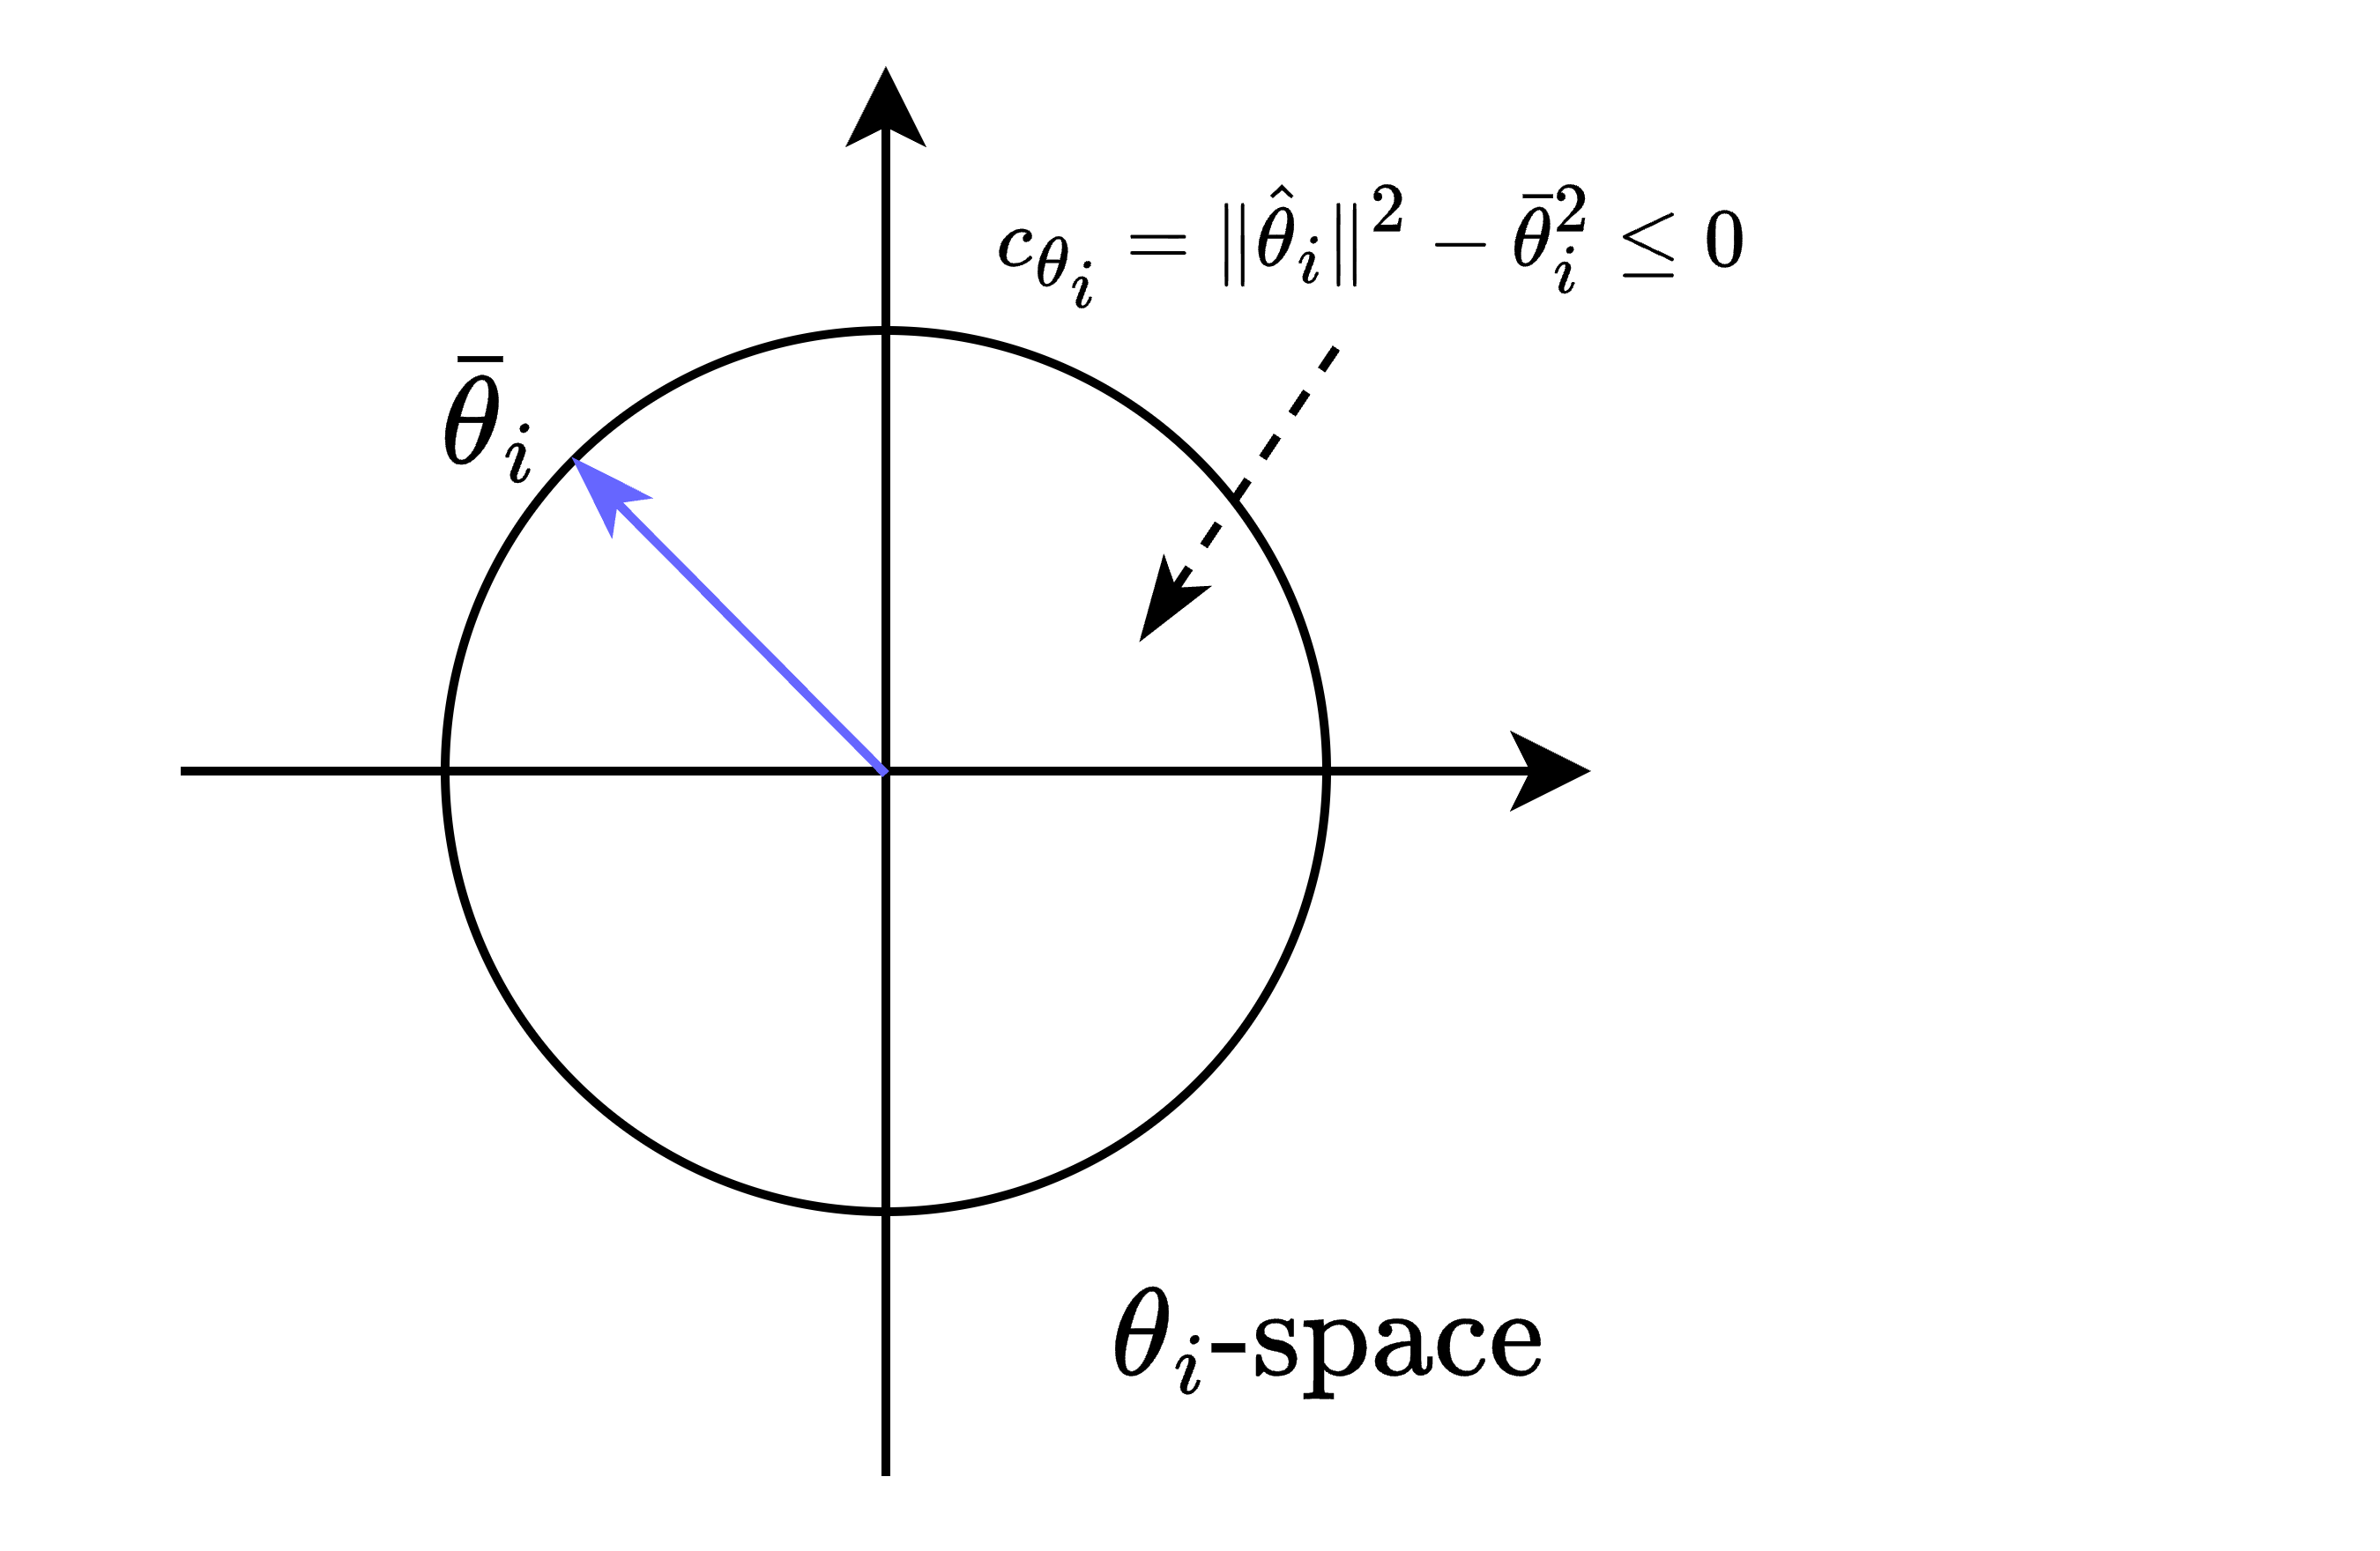
\includegraphics[width=0.5\linewidth]{imgs/cstr_weight.drawio.png}
  \caption{Weight norm constraints.}
  \label{chap3:fig:cstr:weight}
\end{figure*}

The satisfaction of the weights' boundedness is reformulated as a weight norm constraints as shown in Fig.~\ref{chap3:fig:cstr:weight}.
The weight norm constraints are represented as follows:
\begin{equation}
    \begin{aligned}
        c_{\theta_1}(\hat\theta) &\triangleq \Vert \hat\theta_1\Vert^2 - \bar\theta_1^2 \le 0,\\
        c_{\theta_0}(\hat\theta) &\triangleq \Vert \hat\theta_0\Vert^2 - \bar\theta_0^2 \le 0,
    \end{aligned}
    \label{chap3:eq:cstr:weight}
\end{equation}
where $\bar\theta_i^2\in\R_{>0}$ denotes the predefined weight norm bound for each layer $i\in[0,1]$.

The gradient of the constraints can be obtained easily as follows:
\begin{equation}
  \frac{\partial c_{\theta_0}}{\partial\hat\theta}
  = 
  \begin{bmatrix}
      0_{\Xi_1\times 1} \\
      2\hat\theta_0 
  \end{bmatrix}
  ,\quad
  \frac{\partial c_{\theta_1}}{\partial\hat\theta}    
  = 
  \begin{bmatrix}
      2\hat\theta_1 \\
      0_{\Xi_0\times 1}
  \end{bmatrix}
  .
  \label{chap3:eq:cstr:weight_grad}
\end{equation}

%%%%%%%%%%%%%%%%%%%%%%%%%%%%%%%%
\section{Stability Analysis}
%%%%%%%%%%%%%%%%%%%%%%%%%%%%%%%%

The following theorem proves the boundedness of the tracking error and the weight estimation of the weights.

\begin{theorem}
    For the dynamical system in \eqref{chap3:eq:sys1}, the proposed controller \eqref{chap3:eq:approx_control} and the adaptation law \eqref{chap3:eq:adap} ensure the boundedness of the tracking error $\xi$ and the weight estimation $\hat\theta$, provided that control gains ${k_q}$ and ${k_z}$ satisfy \eqref{chap3:eq:stable_cond}.
\end{theorem}

\begin{proof}

The boundedness will be proved from the last layer to the first layer.

\subsubsection{Step 1: Boundedness of $\hat\theta_1,\eta_1,\xi$}

For convenience, assume that all constraints are in the active set without loss of generality.
If the constraints are not in the active set, the boundedness cannot be guaranteed, but weights will be adapted to reduce the objective function until the constraints are violated.

The dynamics of $\xi$ can be represented as
\begin{equation}    
    \dot \xi = A_\xi\xi +B_\xi
    (
        -\hat V_1^T \hat\phi+w(t)
    )
\end{equation}
where $w(t)\triangleq V_1^{*T}\phi^*+\epsilon$ is a lumped residual term, which is bounded as $\Vert w(t)\Vert\le \bar w< 0$.
On the other hand, the dynamics of $\eta_1$ and $\hat\theta_1$ are represented as
\begin{equation}
    \begin{aligned}
        \dot\eta_1 =
        & 
        A_\xi \eta_1 -B_\xi (I_{l_{2}}\otimes \hat\phi^T)
        \\
        \dot{\hat\theta}_1 =
        & -\alpha 
        (
            \eta_1^TW\xi+2\lambda_{\theta_1} \hat\theta_1
        ).
    \end{aligned} 
\end{equation}
According to Theorem \ref{chap2:thm:BIBO}, the boundedness of $\eta_1$ can be obtained, since $A_\xi$ is stable and the residual term $-B_\xi (I_{l_{2}}\otimes \hat\phi^T)$ is bounded.

Define the Lyapunov function $\mathcal V_1=(1/2)\xi^TP\xi+(1/2\alpha)\tilde\theta_1^T\tilde\theta_1$, with the Lyapunov equation $A_\xi^TP+PA_\xi=-Q$, where $A_\xi<0,P=P^T>0$, and $Q>0$.
Using Proposition \ref{chap2:prop:kron} (\ie $\hat V_1^T\hat\phi = \text{vec}(\hat V_1^T\hat\phi)=\text{vec}(\hat\phi^T\hat V_1) = (I_{l_2}\otimes \hat\theta^T)\text{vec}(\hat V_1)=(I_{l_2}\otimes \hat\phi^T)\hat\theta_1$), the time derivative of $\mathcal V_1$ is
\begin{equation}
    \begin{aligned}
        \dot {\mathcal V}_1 =& {1\over 2}\xi^T(A_\xi^TP+PA_\xi)\xi+\xi ^TP ( -B_\xi\hat V_1^T\hat \phi   +B_\xi w(t) )+\hat\theta_1^T
        \bigg(
            -\eta_1^TW \xi-2\lambda_{\theta_1} \hat\theta_1 
        \bigg)
        \\
        =& -{1\over 2}\xi^TQ\xi -\xi^TPB_\xi(I_{l_2}\otimes \hat\phi^T)\hat\theta_1 +\xi^T\Delta
        -\hat\theta_1^T\eta_1^TW\xi
        -2\lambda_{\theta_1} \hat\theta_1^T\hat\theta_1
        \\
        \le& -(1/2)\lambda_\text{min}(Q)\Vert \xi\Vert ^2
        +\bar\Delta \Vert \xi\Vert  
        +\bar M\Vert \xi\Vert  \Vert \hat\theta_1\Vert
        -2\lambda_{\theta_1}
        \Vert\hat\theta_1\Vert ^2
        \\
        \le& 
        \bigg(
        -{\lambda_\text{min}(Q)\over 2} +{\bar M\over 2}
        \bigg)
        \Vert \xi\Vert ^2 +\bar\Delta \Vert \xi\Vert  
        + 
        \bigg(
        -2\lambda_{\theta_1} 
        +{\bar M\over 2}
        \bigg)
        \Vert \tilde\theta_1\Vert ^2 
        \end{aligned}
        \label{chap3:eq:V1_dot}
\end{equation}
where $\Delta\triangleq PB_\xi w(t)$ and $M\triangleq  -PB_\xi(I_{l_2}\otimes \hat\phi^T)+W\eta_1$ which are bounded such that $\Vert\Delta\Vert\le\bar\Delta<\infty$ and $\Vert M\Vert_F\le \bar M< \infty$, respectively.

By defining $P=I_n$, the eigenvalues of $Q=-A_\xi^T-A_\xi$ are $2k_q$ and $2k_z$, since $A_\xi$ is a skew-symmetric matrix except for the diagonal entries.
According to \eqref{chap3:eq:V1_dot}, if $k_q$ and $k_z$ are provided that
\begin{equation}
    \text{min}(k_q,k_z)>\bar M/2
    ,
    \label{chap3:eq:stable_cond}
\end{equation}
and if $\lambda_{\theta_1}$ is increased sufficiently large such that $2\lambda_{\theta_1}>\bar M/2$, due to the violation of the $c_{\theta_1}$, the tracking error is bounded in 
\begin{equation}
    \Theta_\xi = 
    \bigg\{
        \xi \ \bigg\vert\ \Vert\xi\Vert \le  
        {
            \bar \Delta \over \lambda _\text{min}(Q)-\bar M/2
        } 
    \bigg\}
    ,
\end{equation}
and the weight estimation $\theta^*_1$ is bounded in 
\begin{equation}
    \Theta_{\hat\theta_1} = 
    \{ 
        \hat\theta 
        \ 
        \vert
        \ 
        \Vert\hat\theta\Vert \le  
        \bar\theta_1
    \}
    .
\end{equation}
The Lagrange multiplier $\lambda_{\theta_1}$ is also bounded, since $\lambda_{\theta_1}$ update halts once $\hat\theta_1$ approaches into the compact set $\Theta_{\hat\theta_1}$, satisfying the constraint $c_{\theta_1}$.

\subsubsection{Step 2: Boundedness of $\hat\theta_0,\eta_0$}

The dynamics of $\eta_0$ and $\hat\theta_0$ are represented as
\begin{equation}
    \begin{aligned}     
        \dot\eta_0 =& 
        A_\xi\eta_0 -B_\xi 
        \hat V_1^T\hat\phi'(I_1\otimes {q_{NN}}^T)
        \\
        \dot{\hat\theta}_0
        =&
        -\alpha 
        \bigg(
            \eta_0^TW\xi+2\lambda_{\theta_0} \hat\theta_0
        \bigg)
        .
    \end{aligned}
\end{equation}
Also, according to Theorem \ref{chap2:thm:BIBO}, $\eta_0$ is bounded since $A_\xi$ is a stable matrix and $-B_\xi\hat V_1^T\hat\phi'(I_1\otimes {q_{NN}}^T)$ is bounded.
To obtain the invariance set of $\hat\theta_0$, taking the time-derivative of the Lyapunov function $\mathcal V_0=(1/2\alpha)\hat\theta_0^T\hat\theta_0$ yields:
\begin{equation}
    \begin{aligned}
        \dot {\mathcal V}_0 =& 
        \hat\theta_0^T (-\eta_0W\xi -2\lambda_{\theta_0}\hat\theta_0)
        \\
        \le &
        \Vert\hat\theta_0\Vert \Vert \eta_0W\xi\Vert -2\lambda_{\theta_0} \hat\theta_0^T\hat\theta_0
        \\
        \le &
        -2\lambda_{\theta_0} \Vert\hat\theta_0\Vert^2 + \Vert \eta_0W\xi\Vert \Vert \hat\theta_0\Vert 
        .
    \end{aligned}
\end{equation}
Then, the invariance set can be represented as 
\begin{equation}
    \Theta_{\hat\theta_0} =
    \{
        \hat\theta_0\ \vert \ \Vert\hat\theta_0\Vert \le \Vert\eta_0W\xi\Vert/\lambda_{\theta_0}
    \}
    .    
\end{equation}
If $\lambda_{\theta_0}$ is generated sufficiently large due to the violation of $c_{\theta_0}$, the invariance set $\Theta_{\hat\theta_0}$ converges to $\{\hat\theta_0\ \vert \ \Vert\hat\theta_0\Vert \le \bar\theta_0\}$, once the constraint $c_{\theta_0}$ is satisfied. 
Therefore, the Lagrange multiplier $\lambda_{\theta_0}$ is also bounded.

\end{proof}

\begin{remark}
    In the constrained optimization method, the corresponding method of $L_2$-regularization method is the quadratic penalty method, which replaces the constrained optimization problem into an unconstrained optimization problem by adding the penalty term $(1/2\mu)\sum_{r\in\mathcal A} c_r^2$ in the objective function.
    The penalty parameter $\mu\in\R_{>0}$ usually decreases over implementation for the convergence of the optimization process.
    However, the decreased penalty term $\mu$ may alter the original objective function as the penalty term dominates the objective function.
    Therefore, $L_2$-regularization inherently has the analogous drawback of the quadratic penalty method in the selection of the regularization coefficient $\lambda$.
\end{remark}

%%%%%%%%%%%%%%%%%%%%%%%%%%%%%%%%
\section{Simulation Validation}
%%%%%%%%%%%%%%%%%%%%%%%%%%%%%%%%

\subsection{Setup}

\begin{figure}[!t]
    \centering
    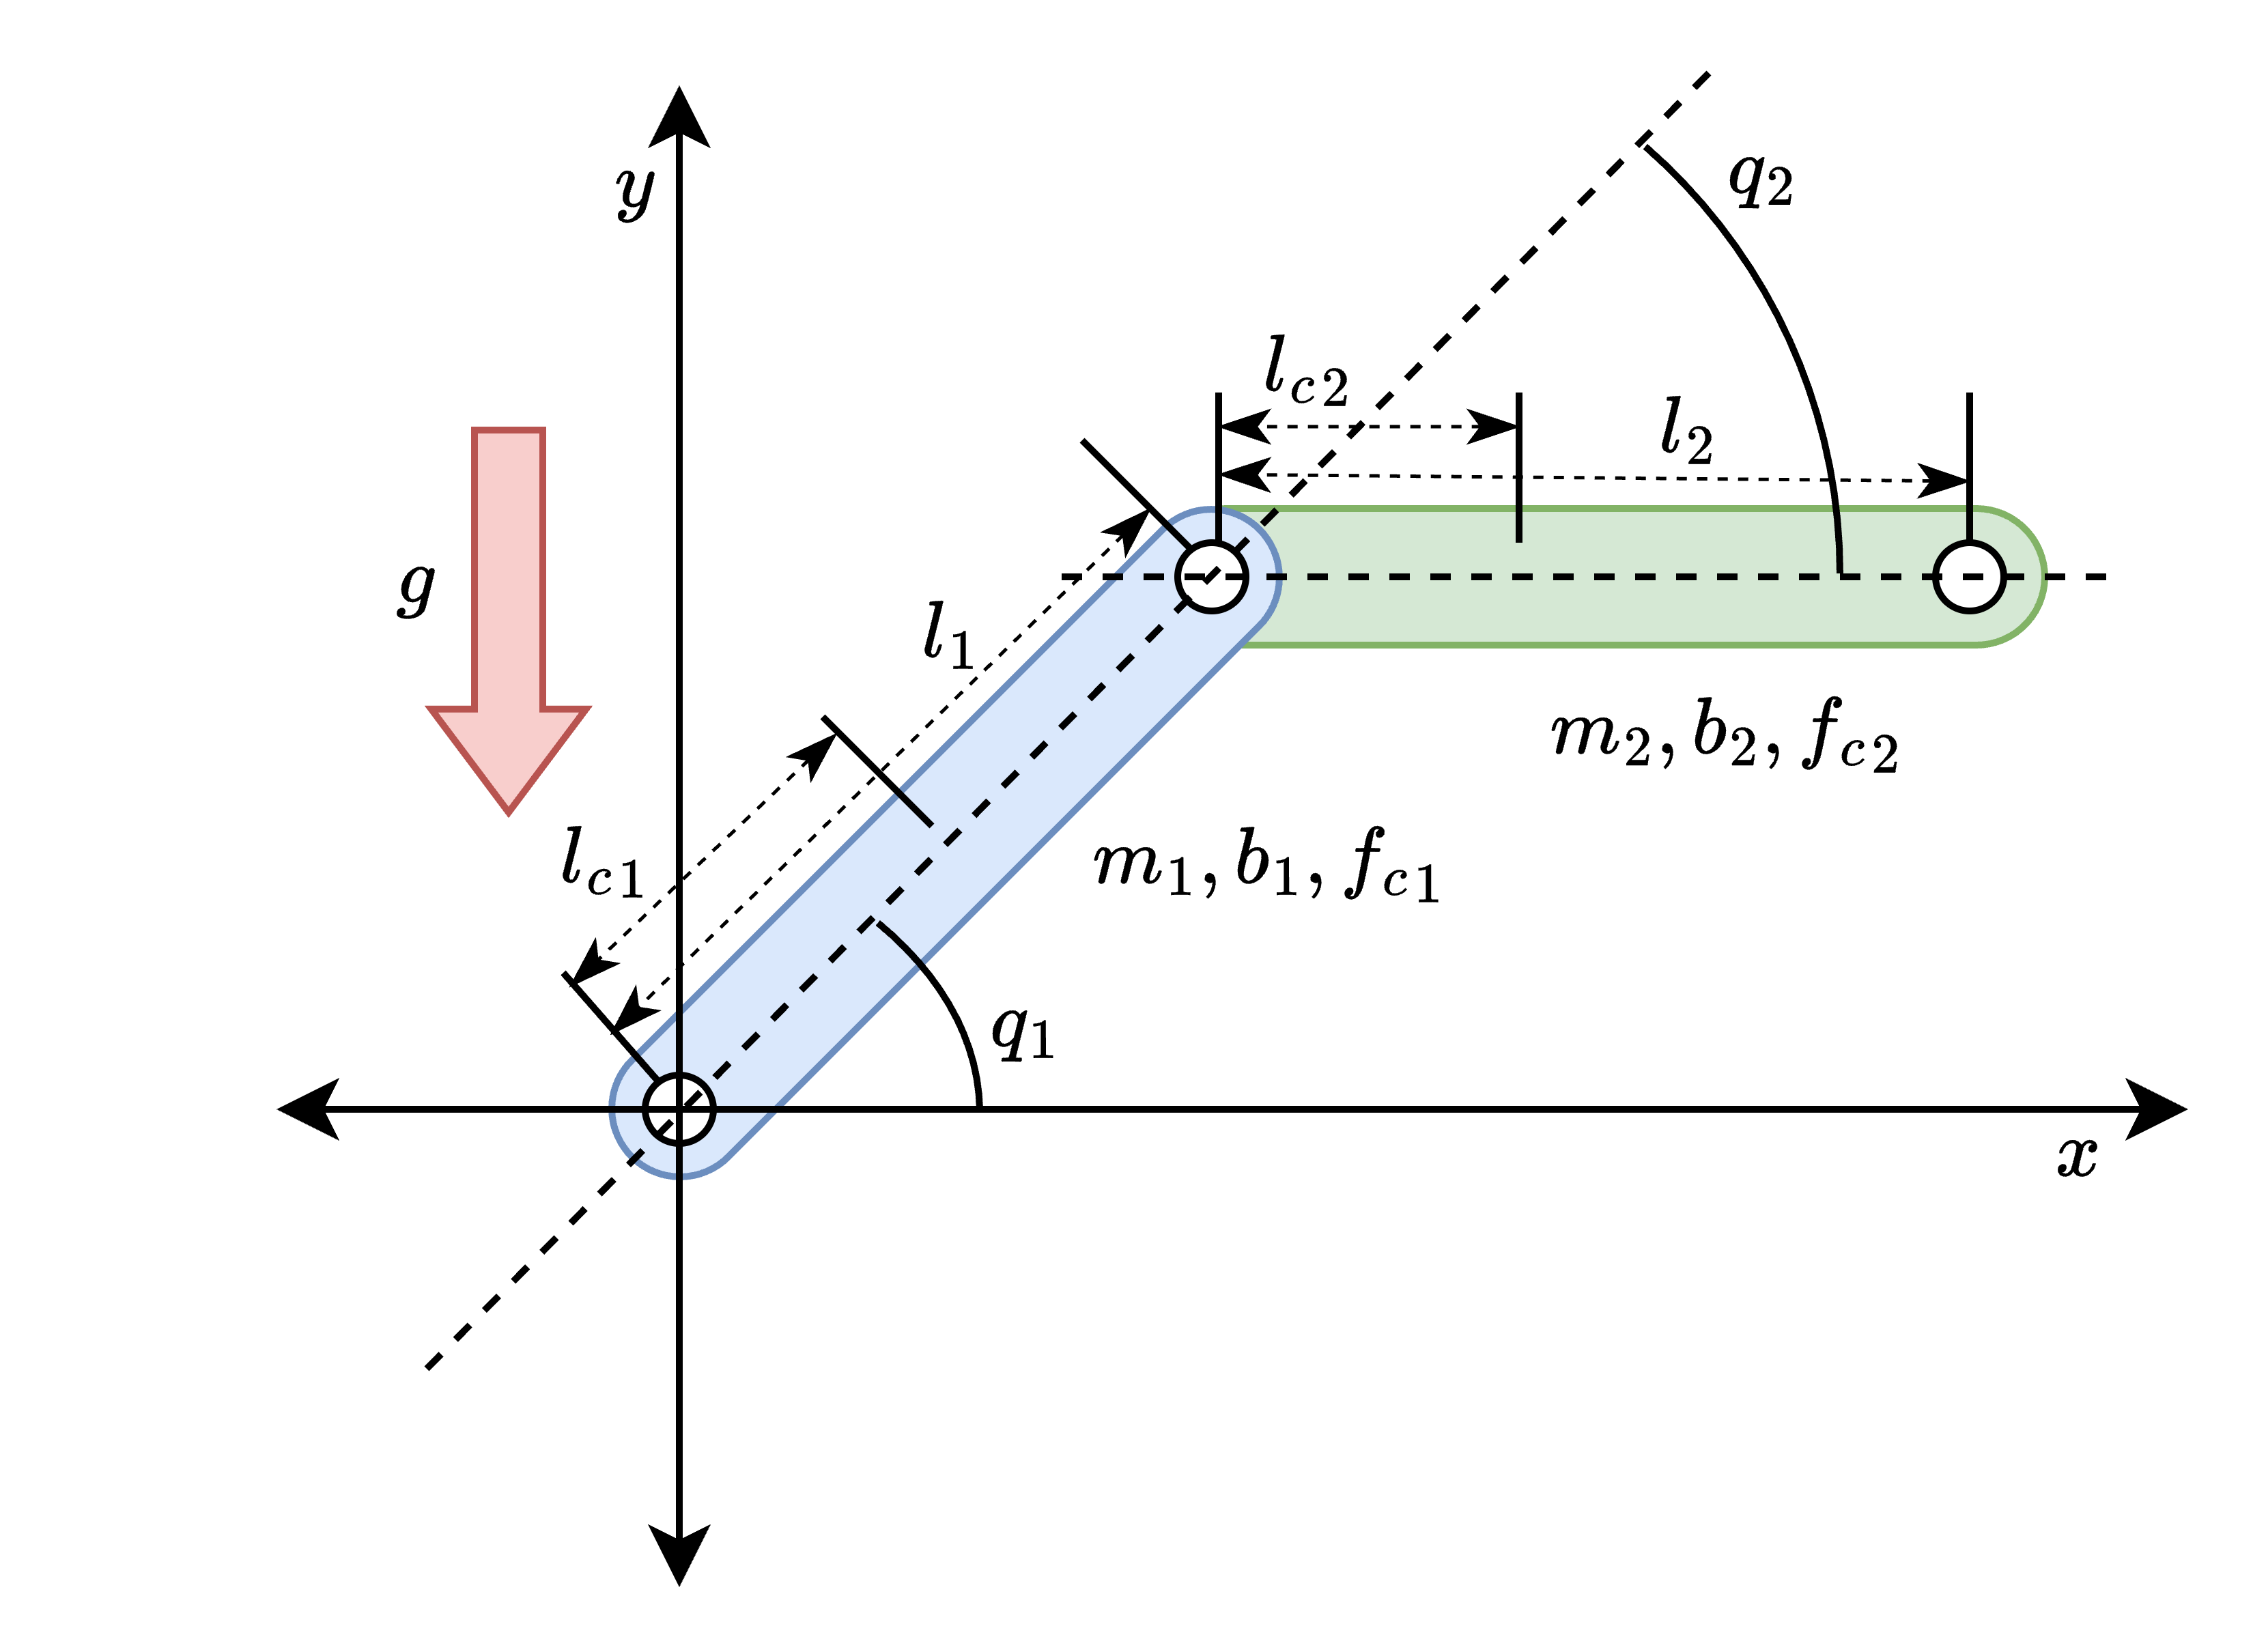
\includegraphics[width=0.75\linewidth]{imgs/RobotModel.drawio.png}
    \caption{Two-link manipulator model.}
    \label{chap3:fig:plant}
\end{figure}

\begin{table}[!t]
    \renewcommand{\arraystretch}{1.3}
    \caption{System model parameters.}
    \centering
    \begin{tabular}{|c||c|c|c|c|}
    \hline
    Symbol & \textbf{Description} & \textbf{Link 1} & \textbf{Link 2} \\
    \hline 
    $m_1, m_2$ & Mass of link    & 23.902 (kg) & 3.88 (kg) \\
    \hline
    $l_1, l_2$  & Length of link   & 0.45 (m) & 0.45 (m) \\
    \hline
    $l_{c1}, l_{c2}$ & COM of link  & 0.091 (m) & 0.048 (m) \\
    \hline
    $\theta_1, b_2$   & Viscous coefficient  &  2.288 (Nms) & 0.172 (Nms) \\
    \hline
    $f_{c1}, f_{c2}$  & Friction coefficient &  7.17 (Nm) & 1.734 (Nm) \\
    \hline
    \end{tabular}
    \label{chap3:table:plant_param}
\end{table}

The two-link manipulator model in \cite{RN33} is employed for the simulation demonstration.
In the system, the parameters $q_p,{q_d}_p,\tau_p,m_p,l_p,{l_c}_p,b_p$, and ${f_c}_p$ denote the joint angle, desired joint angle, torque, mass, length, center of mass, viscous coefficient, and friction coefficient, respectively, for link $p\in[1,2]$.
The values of the system parameters are given in Table~\ref{chap3:table:plant_param}.
The reference signal of the $q=[q_1,q_2]^T$ is defined as follows:
\begin{equation}
    q_d
    =
    \begin{bmatrix}
        {q_d}_1\\
        {q_d}_2
    \end{bmatrix}
    = 
    \begin{bmatrix}
        +\cos(\pi/2 t) + 1 \\
        -\cos(\pi/2 t) - 1 
    \end{bmatrix}
    .
\end{equation}

For the comparative study, three controllers were selected: the neuro-adaptive controller with $L_2$-regularization (NAC-L2) and with $\epsilon$-modification (NAC-eMod), and the proposed controller with constrained optimization (CoNAC).
%%%%%%%%%%%%%%%%%%%%%
The performances of the selected controllers are compared based on the tracking performances and the dependencies of the parameters $\lambda$, $\rho$, and $\beta_j$ of NAC-L2, NAC-eMod, and CoNAC, respectively.
The square root of integrated squared error (ISE) (\ie $\sqrt{\int_0^T\Vert\xi\Vert^2\,dt}$, where $T$ denotes a simulation termination time) is utilized to evaluate the tracking performances.
The parameter dependencies of the controllers were examined via various values of the parameters. 
The values ranged from $0.001$ to $1$ across $10$ samples.
%%%%%%%%%%%%%%%%%%%%%

The control laws of all three controllers were the same as defined in \eqref{chap3:eq:approx_control}.
The adaptation law of NAC-L2 is derived by adding the squared weight term $(1/2)\lambda\hat\theta^T\hat\theta$ to the objective function such that $J_{L_2} = J+(1/2)\lambda\hat\theta^T\hat\theta$, where $\lambda\in\R_{>0}$ denotes the $L_2$-coefficient.
The adaptation law obtained via the gradient descent method is subsequently adjusted by adding stabilizing term $-\alpha\lambda\hat\theta$ as follows:
\begin{equation} 
    \dot{\hat\theta} = 
    {\partial J_{L_2}\over\partial \hat\theta}
    =-\alpha
    \bigg(
        {\partial J\over\partial \hat\theta}+\lambda\hat\theta
    \bigg)
    .
    \label{chap3:eq:adap_L2}
\end{equation}
Note that this adaptation law derived based on $L_2$-regularization method in deep learning is inherently the same as $\sigma$-modification in the adaptive control theory which adds the term $-\alpha\sigma\hat\theta$, where $\sigma\in\R_{>0}$.
For NAC-eMod, Similar to $\sigma$-modification, the stabilizing function $-\alpha\rho\Vert \tilde z \Vert\hat\theta$ is added to the adaptation law as follows:
\begin{equation}
    \dot{\hat\theta} = -\alpha
    \bigg(
        {\partial J\over\partial \hat\theta}+\rho\Vert\tilde z\Vert\hat\theta
    \bigg)
    \label{chap3:eq:adap_eMod}
\end{equation}
where $\rho\in\R_{>0}$ denotes the $\epsilon$-modification coefficient.
By $\Vert\tilde z\Vert$, the stabilizing function proportionally increases as the tracking error $\tilde z$ increases.
Therefore, the adaptation attempts to reduce the tracking error mainly without the effect of the stabilizing function, if the tracking error is sufficiently regulated.
The adaptation law of CoNAC is presented in \eqref{chap3:eq:adap}.
Owing to the stabilizing functions, the weights of NAC-L2 and NAC-eMod are biased, since the stabilizing functions drive the weights toward the origin.

All controllers had the same control parameters except their crucial parameters (\ie $\lambda$, $\rho$ and $\beta_j$) as $k_q=1.1$, $k_z=10$, $M_0=I_2$ and $W=\text{diag}([5,1,15,15])$.
The parameters of the NNs were set $l_0=2$, $l_1=16$, $l_2=2$, and $\alpha=10^3$ and the same random seed was applied for the weight initialization.
The NN input vector was set to the desired trajectory $q_d$, with the augmented 1 to incorporate the bias term in the weight matrix, such that $q_{NN}=[q_d^T,1]^T$. 
For CoNAC, the parameters of the weight norm constraints were set as $\bar\theta_0=10$ and $\bar\theta_1=20$.
The sampling time of the simulation and the simulation termination time were set to $T_s=10^{-4}$ and $T=10$, respectively.

\subsection{Results}

\begin{figure}[!t]      
    \centering
    {\includegraphics[width=.85\linewidth]{imgs/BoxWhisker.drawio.png}}
    \caption{
        Box-and-Whisker plot of the square root of the tracking ISEs of NAC-L2, NAC-eMod and CoNAC across various parameter values.
    }
    \label{chap3:fig:box-whisker}
\end{figure}

\begin{table}[!t]
    \renewcommand{\arraystretch}{1.3}
    \caption{Quantitative comparison of square root of tracking ISE.}
    \centering
    \begin{tabular}{|c||c|c|c|}
    \hline
     & \textbf{NAC-L2} & \textbf{NAC-eMod} & \textbf{CoNAC} (proposed) 
     \\
    \hline 
    Maximum         & $11.1753$e-3 & $0.5603$e-3 & $0.3439$e-3 \\
    \hline
    Upper quartile  & $1.7284$e-3 & $0.5566$e-3 & $0.3261$e-3 \\
    \hline
    Median          & $0.5898$e-3 & $0.5519$e-3 & $0.3240$e-3 \\
    \hline
    Lower quartile  & $0.5533$e-3 & $0.5470$e-3 & $0.3238$e-3 \\
    \hline
    Minimum         & $0.5434$e-3 & $0.5434$e-3 & $0.3235$e-3 \\
    \hline
    \end{tabular}
    \label{chap3:table:error_norm}
\end{table}

As shown in Fig.~\ref{chap3:fig:box-whisker}, the maximum square root of tracking ISE of CoNAC is smaller than the minimum square root of tracking ISEs of NAC-L2 and NAC-eMod for all variations of the parameters.
This is because NAC-L2 and NAC-eMod bias the weights to the origin, due to the presence of the stabilizing functions.
A quantitative comparison of the square root of tracking ISE is provided in Table~\ref{chap3:table:error_norm}.

\begin{figure}[!t]      
    \centering
        \subfloat[NAC-L2]{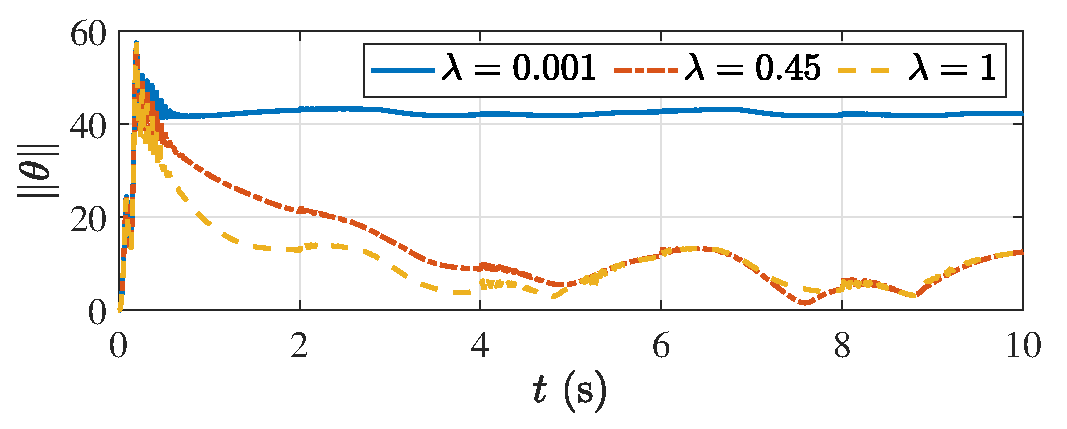
\includegraphics[width=.85\linewidth]{imgs/Chap3/fig9.eps}%
        \label{chap3:fig:weight_NAC-L2}}
    \vfill
        \subfloat[NAC-eMod]{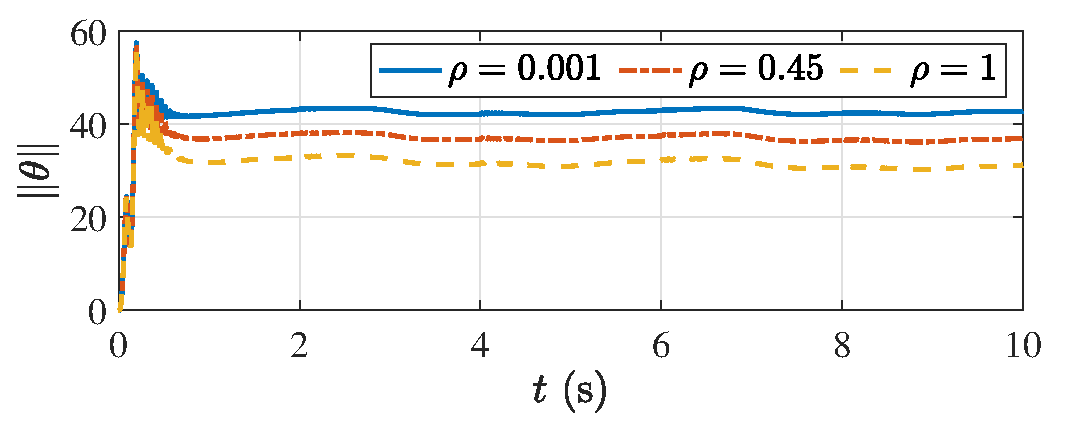
\includegraphics[width=.85\linewidth]{imgs/Chap3/fig10.eps}%
        \label{chap3:fig:weight_NAC-eMod}}
    \vfill
        \subfloat[CoNAC]{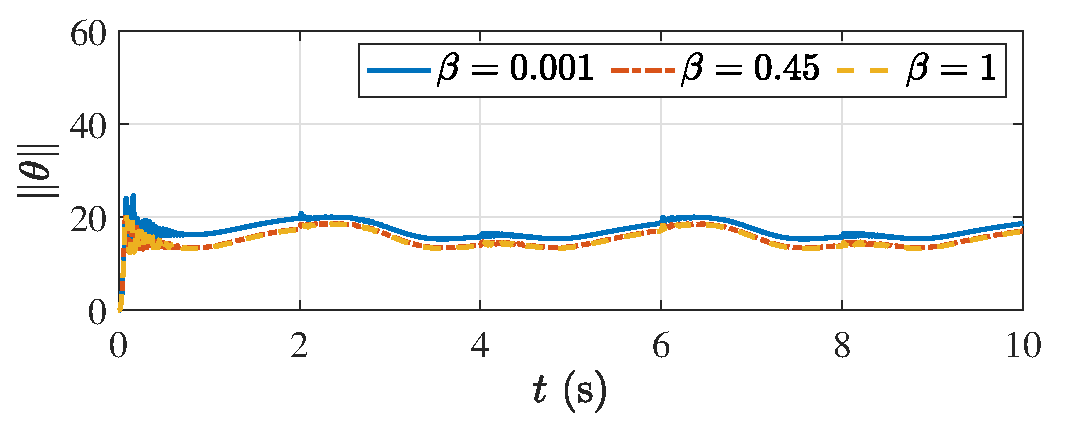
\includegraphics[width=.85\linewidth]{imgs/Chap3/fig8.eps}%
        \label{chap3:fig:weight_CoNAC}}
    \vfill
    \caption{Weight norms of NAC-L2, NAC-eMod and CoNAC.}
    \label{chap3:fig:weight}
\end{figure}

\begin{figure}[!t]      
    \centering
        \subfloat[NAC-L2]{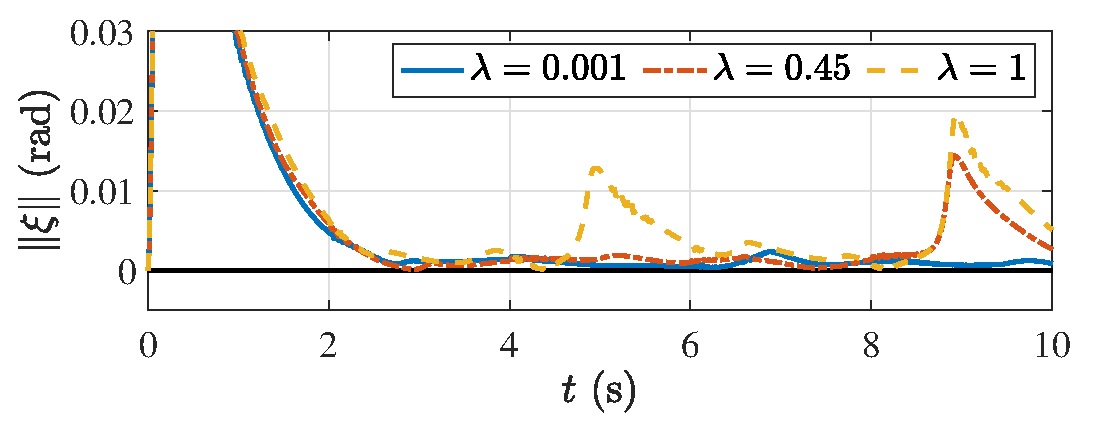
\includegraphics[width=.85\linewidth]{imgs/Chap3/fig6.eps}%
        \label{chap3:fig:error_NAC-L2}}
    \vfill
        \subfloat[NAC-eMod]{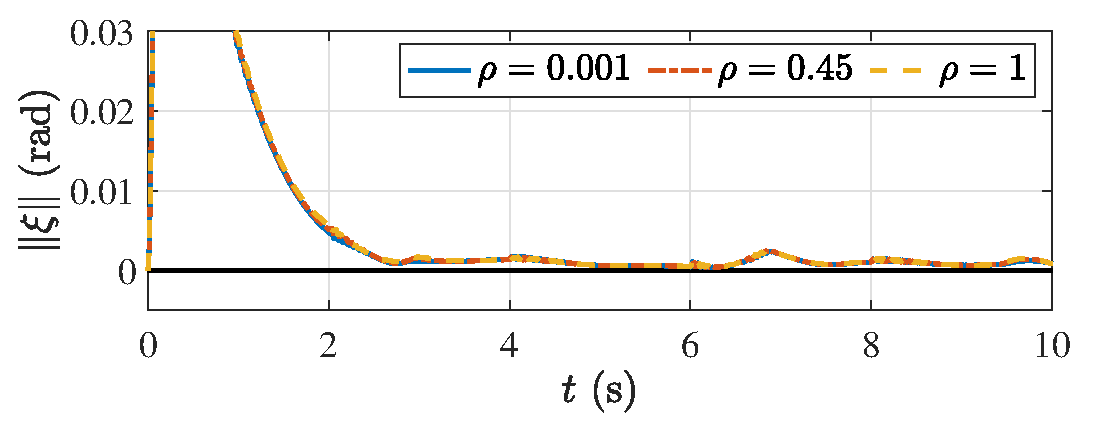
\includegraphics[width=.85\linewidth]{imgs/Chap3/fig7.eps}%
        \label{chap3:fig:error_NAC-eMod}}
    \vfill
        \subfloat[CoNAC]{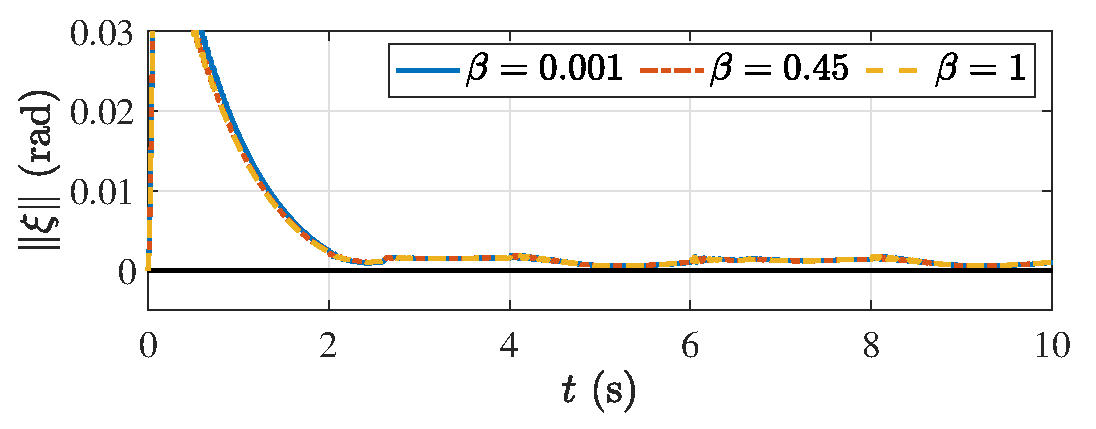
\includegraphics[width=.85\linewidth]{imgs/Chap3/fig5.eps}%
        \label{chap3:fig:error_CoNAC}}
    \vfill
    \caption{Tracking errors of NAC-L2, NAC-eMod and CoNAC.}
    \label{chap3:fig:error}
\end{figure}

For the detailed analysis, three values of the parameters (\ie $\lambda,\rho,\beta_j\in[0.001,0.45,1] \allowbreak $) were selected as described in Fig.~\ref{chap3:fig:weight} and Fig.~\ref{chap3:fig:error}.
As shown in Fig.~\ref{chap3:fig:weight_NAC-L2}, increasing $\lambda$ reduces the weight norm of NAC-L2 by the stabilizing function $-\alpha\lambda\hat\theta$.
Moreover, the high dependency of NAC-L2 to the $L_2$-regularization coefficient $\lambda$ also can be observed.
Since the weight norm is decreased, NAC-L2 cannot generate sufficient control inputs, resulting in a larger square root of tracking ISE, as shown in Fig.~\ref{chap3:fig:error_NAC-L2}.

On the other hand, NAC-eMod exhibits lower dependency on the $\epsilon$-modification coefficient $\rho$ as shown in Fig.~\ref{chap3:fig:weight_NAC-eMod} and Fig.~\ref{chap3:fig:error_NAC-eMod}.
This is because stabilizing function $-\alpha\rho\Vert\tilde z\Vert\hat\theta$ can be decreased once the tracking error $\tilde z$ is sufficiently regulated.
However, the bias of the weights to the origin still exists as described in Fig.~\ref{chap3:fig:weight_NAC-eMod} (\ie smaller weight norms are observed as $\rho$ is increased.).
Therefore, similar to NAC-L2, the biased weights produce insufficient control input, resulting in a relatively larger square root of tracking ISE than that of CoNAC, as described in Table \ref{chap3:table:error_norm}.

Finally, the weight norm of CoNAC is smaller than those of NAC-L2 and NAC-eMod as shown in Fig.~\ref{chap3:fig:weight_CoNAC} with better tracking performances.
Even if the large $\beta_j$ is provided, CoNAC can adjust the adaptation direction to satisfy the weight norm constraints faster, according to \eqref{chap3:eq:adap_L}.
Therefore, the lowest dependency on the update rate $\beta_j$ is observed in CoNAC as shown in Fig.~\ref{chap3:fig:weight_CoNAC} and Fig.~\ref{chap3:fig:error_CoNAC}.
Note that $\beta_j$ of CoNAC is the update rate for Lagrange multipliers while $\lambda$ and $\rho$ are the coefficients of the stabilizing function that generates the biases of the weights.
However, considering the implementation using a digital computer, excessively large $\beta_j$ should be avoided.

The details of the satisfaction of the weight norm constraints are shown in Fig.~\ref{chap3:fig:weight_multiplier CoNAC} for CoNAC with $\beta_j=0.001$.
As the weight norms of each layer reach the constraint boundary, the corresponding Lagrange multipliers are generated.
Using the Lagrange multipliers, the adaptation direction is adjusted toward the constraint satisfactory point.
The Lagrange multipliers disappear when the constraints are satisfied, and the weights are adapted to optimize the original objective function without weight bias.

\begin{figure}[!t]      
    \centering
    \subfloat[Weight norm]{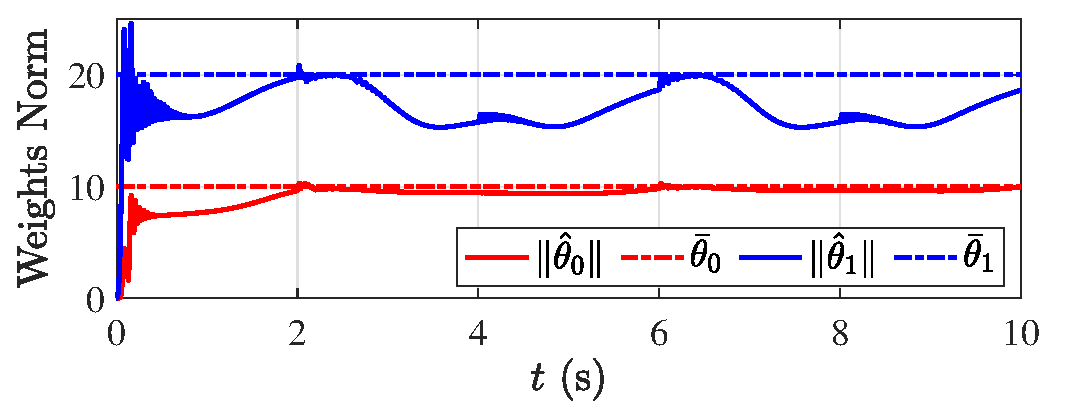
\includegraphics[width=.85\linewidth]{imgs/Chap3/fig12.eps}%
    \label{chap3:fig:weight_norms CoNAC}}
    \vfill
    \subfloat[Lagrange multipliers]{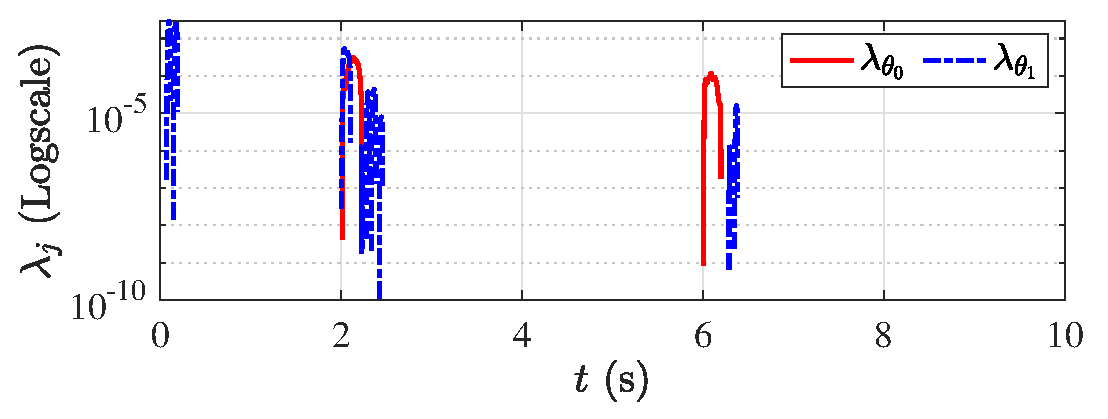
\includegraphics[width=.85\linewidth]{imgs/Chap3/fig11.eps}%
    \label{chap3:fig:multipliers CoNAC}}
    \caption{Weight norms and Lagrange multipliers of CoNAC ($\beta=0.001$).}
    \label{chap3:fig:weight_multiplier CoNAC}
\end{figure}

Furthermore, it is important to note that CoNAC shows enhanced tracking performance with smaller weights than NAC-L2 and NAC-eMod.
This implies that the weights in CoNAC approach the different local optimal solution points from those of NAC-L2 and NAC-eMod.
Therefore, if the physical analysis of the system is available to predict the feasible maximum control inputs, CoNAC can find the local optimal solution without unnecessary large control input by imposing the proper weight norm constraints.

%%%%%%%%%%%%%%%%%%%%%%%%%%%%%%%%
\section{Conclusion}
%%%%%%%%%%%%%%%%%%%%%%%%%%%%%%%%

In this chapter, the CoNAC with SHLNN and weight norm constraint is presented for the uncertain Euler-Lagrange systems.
The boundedness of the weights is handled by formulating a constrained optimization problem with weight norm inequality constraints.
Using the constrained optimization approach, the adaptation laws of the weights and Lagrange multipliers are derived.
The boundedness of the tracking error and the weight estimation are analyzed via Lyapunov analysis.
The simulation results demonstrated that the proposed controller outperforms the existing methods in terms of tracking performance and parameter dependency.
In next chapter, CoNAC will be extended to handle input constraints and DNN.

